\subsection*{Движение по периметру}
\addcontentsline{toc}{subsection}{Движение по периметру}

\textbf{Задание:}\\
Реализовать в среде AnyLogic движение по периметру.\\

\textbf{Решение:}\\
Построим квадрат в качестве поля и красный квадрат в качестве объекта, который будет двигаться по внешнему квадрату. (Рисунок \ref{fig:moving_rectangle1})
\begin{figure}[h]
	\centering 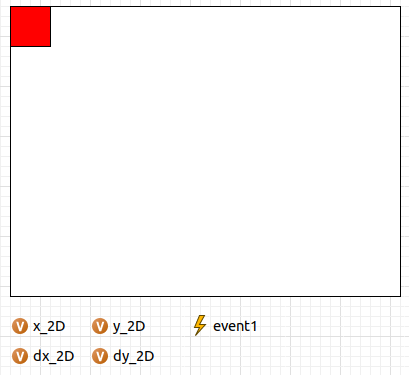
\includegraphics[scale=0.5]{moving_rectangle1}
	\caption{Схема модели в AnyLogic}
	\label{fig:moving_rectangle1}
\end{figure}

Для решения данной задачи нужно завести переменную $x$, которая будет отвечать за текущие координаты квадрата по оси $X$ и переменную $y$, которая будет отвечать за текущие координаты квадрата по оси $Y$. Также потребуются переменные $dx$ и $dy$, которые отвечают за направление движения квадрата. В событии стоит прописать следующий код. (Рисунок \ref{fig:moving_rectangle2})
(Рисунок \ref{fig:moving_rectangle2})
\begin{figure}[h]
	\centering 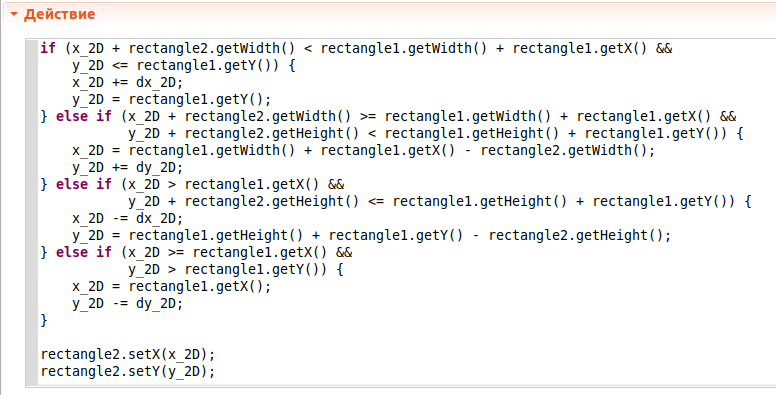
\includegraphics[scale=0.35]{moving_rectangle2}
	\caption{Алгоритм события движения прямоугольника по периметру}
	\label{fig:moving_rectangle2}
\end{figure}

Получается, что если мы дошли до какой-то из границ внешнего квадрата, то мы просто меняем направление движения и обновляем координаты красного квадрата.\\

Подводя итог, нам удалось воспроизвести необходимые типы движения и познакомится с примерами работы с элементами презентации.\\